%%%%%%%%%%%%%%%%%%%%%%%%%%%%%%%%%%%%%%%%%
% fphw Assignment
% LaTeX Template
% Version 1.0 (27/04/2019)
%
% This template originates from:
% https://www.LaTeXTemplates.com
%
% Authors:
% Class by Felipe Portales-Oliva (f.portales.oliva@gmail.com) with template 
% content and modifications by Vel (vel@LaTeXTemplates.com)
%
% Template (this file) License:
% CC BY-NC-SA 3.0 (http://creativecommons.org/licenses/by-nc-sa/3.0/)
%
%%%%%%%%%%%%%%%%%%%%%%%%%%%%%%%%%%%%%%%%%

%----------------------------------------------------------------------------------------
%	PACKAGES AND OTHER DOCUMENT CONFIGURATIONS
%----------------------------------------------------------------------------------------

\documentclass[
	english,
	11pt, % Default font size, values between 10pt-12pt are allowed
	%letterpaper, % Uncomment for US letter paper size
	%spanish, % Uncomment for Spanish
]{fphw}

% Template-specific packages
\usepackage{babel}
\usepackage[utf8]{inputenc} % Required for inputting international characters
\usepackage[T1]{fontenc} % Output font encoding for international characters
\usepackage{mathpazo} % Use the Palatino font
% \usepackage{iwona}    %% Roman text font 
% \usepackage{mathdots}
% \usepackage{eulervm}
% \usepackage{iwona} % Use the Iwona font

\usepackage{amsmath}
\usepackage{mathtools}
\usepackage{cases}	% Required to use nmbered tags in cases

\usepackage{graphicx} % Required for including images
\usepackage[justification=centering]{caption}  %% To manage long captions in images
\usepackage{subcaption}
\usepackage{float}
\graphicspath{ {./img/} }

\usepackage{booktabs} % Required for better horizontal rules in tables

\usepackage{listings} % Required for insertion of code

\usepackage{array} % Required for spacing in tabular environment

\usepackage{enumerate} % To modify the enumerate environment

\usepackage{amssymb}
\usepackage{enumitem}	%% % To modify the itemize bullet character

\usepackage[linkcolor=blue,colorlinks=true]{hyperref}
\usepackage{cleveref}  %% To make links clickable

\newcommand{\hquad}{\hspace{0.5em}} %% Bew command for half quad
\usepackage{indentfirst}	%% Indent the first paragraph
\newcommand{\bi}{\text{Bi}} 
\newcommand{\vertiii}[1]{{\left\vert\kern-0.25ex\left\vert\kern-0.25ex\left\vert #1 
    \right\vert\kern-0.25ex\right\vert\kern-0.25ex\right\vert}}

%----------------------------------------------------------------------------------------
%	ASSIGNMENT INFORMATION
%----------------------------------------------------------------------------------------

\title{Problem Set \#2: RB for Linear Affine Elliptic} % Assignment title

\author{Roussel Desmond Nzoyem} % Student name

\date{\today} % Due date

\institute{University of Strasbourg \\ UFR de Mathématiques et Informatique} % Institute or school name

\class{Calcul Scientifique 3} % Course or class name

\professor{Pr. Christophe Prud'homme} % Professor or teacher in charge of the assignment

%----------------------------------------------------------------------------------------

\begin{document}

\maketitle % Output the assignment title, created automatically using the information in the custom commands above

%----------------------------------------------------------------------------------------
%	ASSIGNMENT CONTENT - SECTION 1
%----------------------------------------------------------------------------------------


% \section*{Reduced Basis Approximation}

\subsection*{Question a)}
\begin{problem}
	Show that the operation count for the on-line stage of your code is independent of N.
\end{problem}

For each step of the online stage, let's count the number of floating point operations (multiplications and additions):
\begin{enumerate}
	\item Form $A_N(\mu)$ from $A_N(\mu)=\sum_{q=1}^Q \Theta^q(\mu)A_N^q$: requires $QN^2$ multiplications, and $(Q-1)N^2$ additions, hence $(2Q-1)N^2$ flops in total
	\item Solve the $N\times N$ linear system $A_N(\mu)u_N(\mu)=F_N$: requires at most $N^3$ flops. In the case of the $LU$ decomposition (where $L$ has $1$'s along its diagonal), the cost of the decomposition is $\frac{2N^3}{3} - \frac{N^2}{2} - \frac{N}{6}$ flops, the cost for the descent algorithm is $N(N+1)$, and the cost for the ascent is $N(N+1)+N$
	\item Evaluate the output $T_{rootN}(\mu)=L_N^Tu_N(\mu)$: requires $2N-1$ flops as a dot product
\end{enumerate}
In conclusion, the operation count for the on-line stage is independent of $\cal{N}$, it is equal to $$(2Q-1)N^2+ \frac{2N^3}{3}-\frac{N^2}{2}-\frac{N}{6} +2N(N+1)+N + 2N-1$$ which yields $$\frac{2}{3}N^3 + (2Q+\frac{1}{2})N^2 + \frac{29}{6}N - 1 $$ roughly equal to $$c_1N^{\gamma_1}+c_2N^{\gamma_2}+c_3N^{\gamma_3}$$ with:
\begin{align*}
	\begin{cases}
		c_1 = \frac{29}{6}, &\quad \gamma_1=1 \\
		c_2 = 2Q+\frac{1}{2},&\quad \gamma_2 = 2 \quad (Q=6)\\
		c_3 = \frac{2}{3},&\quad \gamma_3 = 3
	\end{cases}
\end{align*}

% \subsection*{Answer} 

% ---------------------------------------------------------------
% QUESTION 2
% ---------------------------------------------------------------


\subsection*{Question b)}
\subsubsection*{1}
\begin{problem}
	Generate the reduced basis matrix Z and all necessary reduced basis quantities.
\end{problem}

% \subsection*{Answer} 

For $N=8$, $\mu=1$ and $\mu = 10$, let's compare the condition number of $A_N(\mu)$, noted $\text{Cond}(A_N(\mu))$, when the $Z$ matrix is taken directly from the "snapshots" (No G-S), and when when $Z$ is orthonormalized using the Gram-Schmidt (G-S) process. $\gamma$ and $\alpha$ are respectively the continuity (Lipschitz constant) and the coercivity constants for $A_{\cal{N}}$.
\begin{itemize}
	\item[$\blacksquare$] $\mu=1$:
	\begin{itemize}
		\item \textbf{No G-S}: $\text{Cond}(A_N(\mu)) = 33575189921.6$
		\item \textbf{with G-S}: $\text{Cond}(A_N(\mu)) = 1.0000000000959741$
		\item \textbf{Upper bound}: $\frac{\gamma(\mu)}{\alpha(\mu)} = 1.0000000000000868$
	\end{itemize} 
	\item[$\blacksquare$] $\mu=10$:
	\begin{itemize}
		\item \textbf{No G-S}: $\text{Cond}(A_N(\mu)) = 23018985185.0$
		\item \textbf{with G-S}: $\text{Cond}(A_N(\mu)) = 9.9286$
		\item \textbf{Upper bound}: $\frac{\gamma(\mu)}{\alpha(\mu)} = 10.000$
	\end{itemize} 
\end{itemize}
It can be observed that the condition number is bounded by a function of $\mu$ when the Gram-Schmidt orthonormalization is applied to $Z$ (specifically $\mu \mapsto \frac{1}{\mu}$ if $\mu<1$ and $\mu \mapsto \mu$ if $\mu \geq1$). This fits the results from the previous Problem Set, indicating that $\frac{\gamma(\mu)}{\alpha(\mu)}$ should be an upper bound for $A_N$'s condition number (the upper bound is computed by solving a generalized eigen value problem $ \left(A_{\mathcal{N}}(\mu)-\lambda A_{\mathcal{N}}(\bar{\mu})\right)x = 0$, for $x\in X^e$).  

\textbf{Without orthonormalization}: Since $\mu_1, \mu_2$ were taken as snapshots to build the RB basis, one component of $u_N(\mu_1)$ and $u_N(\mu_2)$ must be equal to $1$ while all the others are close to $0$. This is what is observed. As for $\mu_3 = 1.0975$ which is not in 'sample1', the resulting $u_N(\mu_3)$ doesn't contain $0$'s nor $1$'s. Instead, the result is a combination of all the snapshots in $Z$, inducing a huge loss in accuracy.

\textbf{With orthonormalization}: Here the components in $Z$ that do not count as part of the solution are less pronounced (closer to $0$). For example, since $u_N(\mu_1)$ is the first snapshot, its first component is $1$ and the rest are $0$ (close to the floating point precision). The same result is observed for $u_N(\mu_2)$, which is a combination of the first and second snapshots.

\subsubsection*{2}
\begin{problem}
	Let's verify the output.
\end{problem}


% \subsection*{Answer} 
For $\mu = 1.5$, $\bi = 0.1$, the computed value on a coarse grid is effectively $$T_{rootN}(\mu)=1.531074970789645$$


\subsubsection*{3}
\begin{problem}
	Convergence study over a test sample.
\end{problem}


% \subsection*{Answer} 
Figure \cref{fig:sample1Error} shows the convergence of the maximum
relative error in the energy norm and the maximum relative
output error as a function of N. As expected, it proves the errors decrease as our reduced basis' dimension $N$ increases.

\begin{figure}[H]
	\centering
	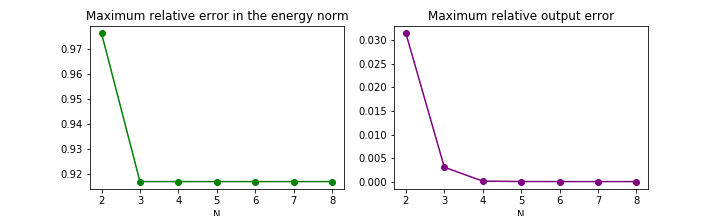
\includegraphics[width=0.95\textwidth]{sample1Error.png}
	\caption{Maximum relative error in the energy norm and the maximum relative output error as a function of N, applied to sample 1. This plot is identical for a coarse, a medium, and fine FE triangulation}
	\label{fig:sample1Error}
\end{figure}


Now let's compare the convergence in energy norm (in $log$ mode) when the matrix Z is (not) orthonormalized. \cref{fig:CompOrth} shows a much faster convergence (and a considerably lower error) when the matrix $Z$ is orthonormalized. This justifies the use of orthonormalization since question $b)1$.
\begin{figure}[H]
	\centering
	\begin{subfigure}[b]{0.45\textwidth}
		\centering
		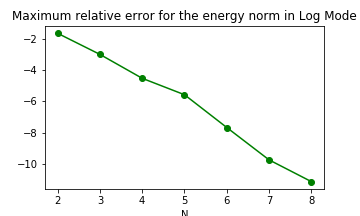
\includegraphics[width=\textwidth]{sample1ErrorLog.png}
		\caption{Without orthonormalization}
	\end{subfigure}
	\begin{subfigure}[b]{0.45\textwidth}
		\centering
		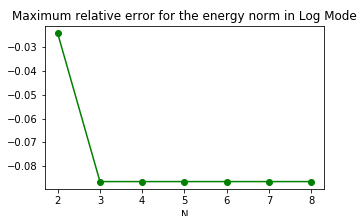
\includegraphics[width=\textwidth]{sample1ErrorLogOrth.png}
		\caption{With orthonormalization}
	\end{subfigure}
	   \caption{Comparison of energy norm error convergence in log mode when the RB matrix $Z$ is orthonormalized, and when it is not.}
	   \label{fig:CompOrth}
\end{figure}


\subsubsection*{4}
\begin{problem}
	Average CPU time comparison.
\end{problem}


% \subsection*{Answer} 
From \cref{fig:sample1Times}, the relation between the computation and $N$ cannot easily be deduced. However, it clearly indicates how much faster the reduced basis' online stage is, compared to the finite element's computation of the exact solution. 

\begin{figure}[H]
	\centering
	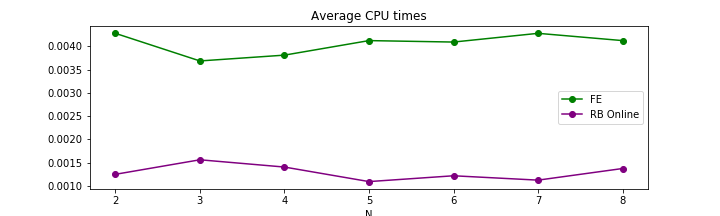
\includegraphics[width=0.7\textwidth]{sample1Time.png}
	\caption{Average CPU time over test sample1 required to solve the reduced basis online stage with direct solution of the FE approximation as a function of $N$. This comparison is only valid on a coarse FE triangulation}
	\label{fig:sample1Times}
\end{figure}


\subsubsection*{5}
\begin{problem}
	Required value of $N$ for a $1\%$ accuracy.
\end{problem}

On a coarse triangulation, as long as $N$ is greater or equal to $2$, we have a relative accuracy of less than $1\%$. Moreover, the average time saving in terms on CPU time (compared to the FE method's computation) is about \textbf{$0.0028125$} seconds.


\subsubsection*{6}
\begin{problem}
	Dependence of $\cal{N}$ on the results.
\end{problem}

Repeating steps 3. to 5. on medium and fine triangulations we get the following results.

\begin{itemize}
	\item[$\blacksquare$] COARSE: 
	\begin{itemize}
		\item Maximum relative errors: see \cref{fig:sample1Error} 
		\item CPU Time comparison: see \cref{fig:sample1Times}
		\item Achieved accuracy: 0.3056515255907647 \%
		\item Required N: 3
		\item CPU time savings: 0.0028645833333333327 sec
	\end{itemize}
	\item[$\blacksquare$] MEDIUM: 
	\begin{itemize}
		\item Maximum relative errors: see \cref{fig:sample1Error} 
		\item CPU Time comparison: see \cref{fig:sample1TimesMedium}
		\item Achieved accuracy: 0.3022017037569751 \%
		\item Required N: 3
		\item CPU time savings: 0.012812499999999998 sec
	\end{itemize}
	\item[$\blacksquare$] FINE: 
	\begin{itemize}
		\item Maximum relative errors: see \cref{fig:sample1Error} 
		\item CPU Time comparison: see \cref{fig:sample1TimesFine}
		\item Achieved accuracy: 0.300010213328605 \%
		\item Required N: 3
		\item CPU time savings: 0.067875 sec
	\end{itemize}
\end{itemize}

\begin{figure}[H]
	\centering
	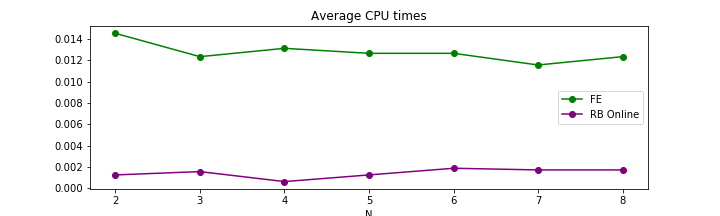
\includegraphics[width=0.7\textwidth]{sample1TimeMedium.png}
	\caption{Average CPU time comparison on a medium FE triangulation}
	\label{fig:sample1TimesMedium}
\end{figure}

\begin{figure}[H]
	\centering
	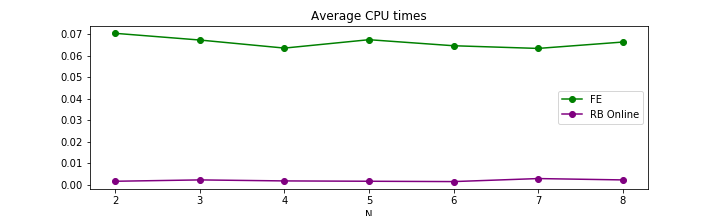
\includegraphics[width=0.7\textwidth]{sample1TimeFine.png}
	\caption{Average CPU time comparison on a fine FE triangulation}
	\label{fig:sample1TimesFine}
\end{figure}

Unsurprisingly, the time required to compute the FE direct solution increases considerably (see \cref{fig:sample1Times,fig:sample1TimesMedium,fig:sample1TimesFine}) while the time required by for the RB approximation is fairly constant around $0.002$ second. This apparent non-dependence on $\cal{N}$ (on the triangulation) is once again observed on the maximum and relative errors in the RB approximation (the same figure (\cref{fig:sample1Error}) for all 3 triangulations).

As for the accuracy, we notice that while the required minimal $N$ most still equal $3$ to have a $1 \%$ output accuracy , the achieved accuracy clearly decreases with $\cal{N}$ for the wanted $N=3$ (a $0 \%$ accuracy means the RB approximation is identical to the exact FE computation). With this output precision increase, the CPU time saved increases. In summary, \textbf{the finer the FE triangulation, the greater the need for a reduced basis approximation}. This is exactly what was expected.  



\subsection*{Question c)}
\subsubsection*{1}

\begin{problem}
	Let's verify the output on $\Gamma_{root}$
\end{problem}

% \subsection*{Answer} 
For $\mu = 0.4, 0.6, 0.8, 1.2, 0.15$, the computed value on a medium grid is effectively $$T_{rootN}(\mu)=1.51561$$


\subsubsection*{2}
\begin{problem}
	Convergence study over a test sample.
\end{problem}

% \subsection*{Answer} 
Figure \cref{fig:sample2Error} shows the convergence of the maximum
relative error in the energy norm and the maximum relative
output error as a function of N.

\begin{figure}[H]
	\centering
	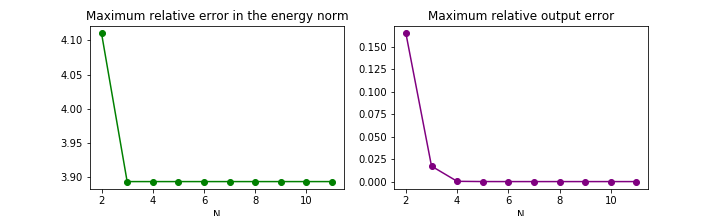
\includegraphics[width=0.95\textwidth]{sample2Error.png}
	\caption{Maximum relative error in the energy norm and the maximum relative output error as a function of N, applied to sample 2.}
	\label{fig:sample2Error}
\end{figure}

We can see that the maximum relative errors in the energy norm and output error condirebably decrease as $N$ gets bigger.


\subsubsection*{3}
\begin{problem}
	Cost minimisation.
\end{problem}

Applying the bisection method with a tolerance of $10^{-16}$, we find that the optimal cost is $C=1.4655$, obtained for the Biot number $\bi = 0.40295$.

\subsection*{Question d)}
\subsubsection*{1}

\begin{problem}
	Convergence study over a test sample.
\end{problem}

% \subsection*{Answer} 
Figure \cref{fig:sample3Error} shows the convergence of the maximum
relative error in the energy norm and the maximum relative
output error as a function of N.

\begin{figure}[H]
	\centering
	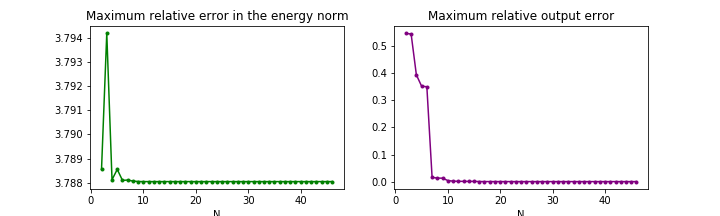
\includegraphics[width=0.95\textwidth]{sample3Error.png}
	\caption{Maximum relative error in the energy norm and the maximum relative output error as a function of N, applied to sample 3.}
	\label{fig:sample3Error}
\end{figure}

As we noticed before, the maximum relative errors in the energy norm and output error decrease as N gets bigger (although not by much). However, when comparing it to \cref{fig:sample1Error,fig:sample2Error}, it it clear that the errors reach quite higher values.


% \clearpage
% -------------------------------------------------------------------------------
% REFERENCES
% --------------------------------------------------------------------------------
% \section*{References}
% \begin{itemize}
% 	\item Legoll, F. (2019). \textit{Partial Differential Equations and the Finite Element Method}. Retrieved from \url{http://cermics.enpc.fr/~legoll/poly_EDP-EF_jan19.pdf}.
% \end{itemize}

\end{document}
